In this section we show results from the \herwigpp, \pythiaeight and \sherpa MC
generators described in \PartRef{sec:spec-revi-main}, compared to data from a
variety of collider experiments from \lep to the \lhc. In all these plots, the
versions and tunes shown are: for \herwigpp, a pre-release copy of version 2.5.0
with the default tune to the MRST~LO$**$ PDF; for \pythiaeight, version 8.145
with tune 4C and the \cteq{6L1} PDF; and for \sherpa, version 1.2.3 with the
default tune and the \cteq{6L1} PDF. All the analyses shown are in \rivet.

It should be emphasised here that the generators have not yet been optimally
tuned to LHC data overall, or indeed to any of the particular plots shown.  The
intention here is rather to give an ``existence proof'' of output from the
programs.  Therefore the success or otherwise of a generator in fitting the data
should not at this stage be taken as a true measure of its performance.  As
stated in the figure captions, as tuning progresses the plots will be updated
and archived at \url{http://mcplots.cern.ch/}.

\FigRef{fig:cmp:intrinsic-kt} shows the $Z^0$ transverse momentum
distribution in $p\bar p$ collisions at $\sqrt s=1.8$ TeV, compared
with CDF data~\cite{Affolder:1999jh}.  As discussed in \SecRef{sec:primkt}, the
position and shape of the peak in this distribution is sensitive to
the modelling of non-perturbative effects generically termed
``primordial \kT''.

In \FigRef{fig:cmp:mpi-minbias} we show results on soft QCD processes
compared with ATLAS minimum bias data~\cite{Atlas:2010xx}.

\FigsRef{fig:cmp:mpi-ue-atlas-1}--\ref{fig:cmp:mpi-ue-atlas-3} show
observables relevant to the underlying event, discussed in
\SecRef{sec:minim-bias-underly}, compared to ATLAS data at 900 GeV
  and 7 TeV~\cite{Aad:2010fh}.  Various indicators of event activity
  are measured in the transverse region, \ie at $60^\circ-120^\circ$ in
  azimuth, relative to the leading-\pt\ charged particle.
\FigRef{fig:cmp:mpi-ue-cdf} shows similar results for the Tevatron, in
the transverse region relative to the leading jet, and in the towards
region, \ie closer than $60^\circ$ in azimuth, relative to the $Z^0$
direction in Drell-Yan events, compared to CDF data~\cite{Aaltonen:2010rm}.

Some results on final states in $e^+e^-$ annihilation at the $Z^0$
peak are shown in
\FigsRef{fig:cmp:eeshapes}--\ref{fig:cmp:eejetrates}, together with
ALEPH data~\cite{Barate:1996fi,Heister:2003aj}.  Other plots relevant to jet
fragmentation are shown in
\FigsRef{fig:cmp:ppshapes}--\ref{fig:cmp:bfragfunction}.

Finally \FigRef{fig:cmp:cdf-colour-coherence} shows results from
the MCnet generators on the colour-coherence test discussed in
\SecRef{parton-shower:initial-conditions} (already displayed in
\FigRef{fig:CDFcoherence} for the earlier generator \pythiasix),
again compared with CDF data~\cite{Abe:1994nj}.

\begin{figure}[tp]
  \centering
  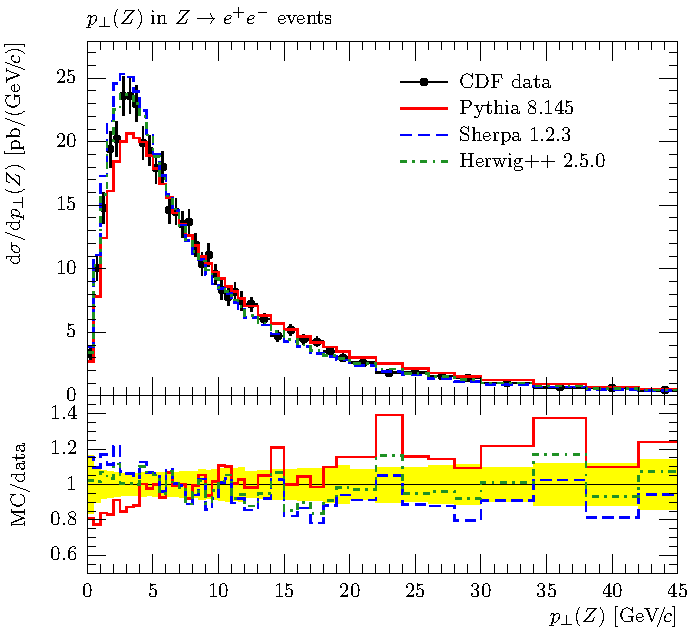
\includegraphics[scale=0.7]{mc-plots/CDF_2000_S4155203-cmp/CDF_2000_S4155203_d01-x01-y01}
  \caption{CDF 2000 $Z^0$ \pT peak \cite{Affolder:1999jh}.  The location
    of the peak is very sensitive to the degree of ``primordial \kT''
    smearing in the generator, and the higher-\pT region is affected by
    the parton shower. In all cases, the generators have been run with
    LO matrix elements, and the MC normalization is fixed to that of the
    data, to alleviate the requirement for an NLO cross-section.  An
    up-to-date version of this plot can be found at
    \url{http://mcplots.cern.ch/}.}
  \label{fig:cmp:intrinsic-kt}
\end{figure}

\begin{figure}[tp]
  \centering
  \subfigure[Charged multiplicity]{\label{fig:cmp:mpi-minbias-atlasnch}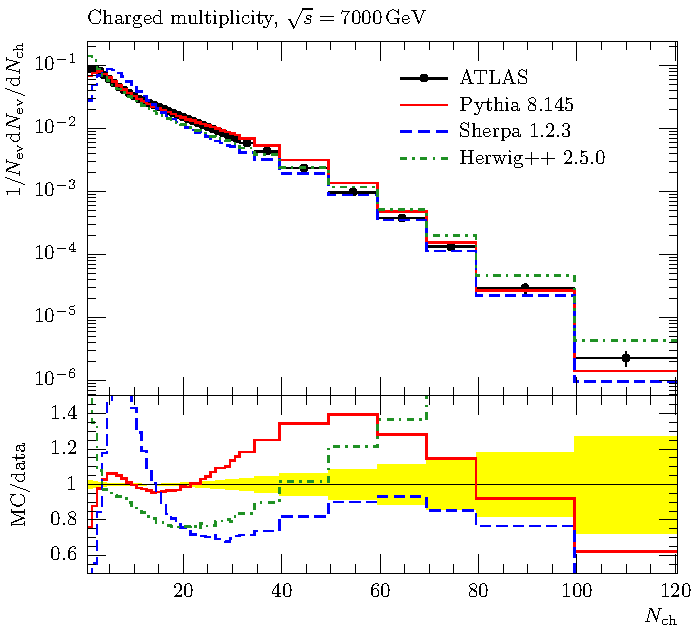
\includegraphics[scale=0.7]{mc-plots/ATLAS_2010_CONF_2010_031-cmp/ATLAS_2010_CONF_2010_031_d03-x02-y01}}
  \subfigure[$\langle \pT \rangle$ vs. $N_\text{ch}$]{\label{fig:cmp:mpi-minbias-atlasptnch}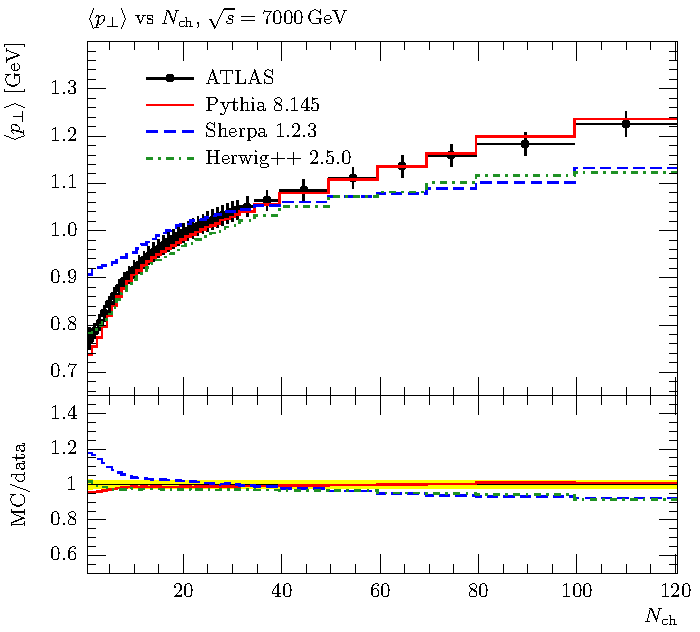
\includegraphics[scale=0.7]{mc-plots/ATLAS_2010_CONF_2010_031-cmp/ATLAS_2010_CONF_2010_031_d03-x04-y01}}
  \caption{ATLAS minimum bias charged particle distributions at 7~TeV,
    with a charged particle \pT cut of $\pT > 500~\text{MeV}$,
    $|\eta| < 2.5$, $c\tau > 10\,\text{mm}$
    \cite{Atlas:2010xx}. The MC description of these observables is
    dominated by the tuning of the MPI models: the inclusive charged
    multiplicity is dependent on the level of MPI activity, and the
    correlation between $\langle \pT \rangle$ and $N_\text{ch}$ is
    affected by colour reconnection, as described in
    \SecRef{sec:minim-bias-underly}. Up-to-date versions of these plots
    can be found at \url{http://mcplots.cern.ch/}.}
  \label{fig:cmp:mpi-minbias}
\end{figure}

\begin{figure}[tp]
  \centering
  \subfigure[Transverse $N_\text{ch}$ at 900~GeV]{\label{fig:cmp:mpi-ue-atlas900-nch}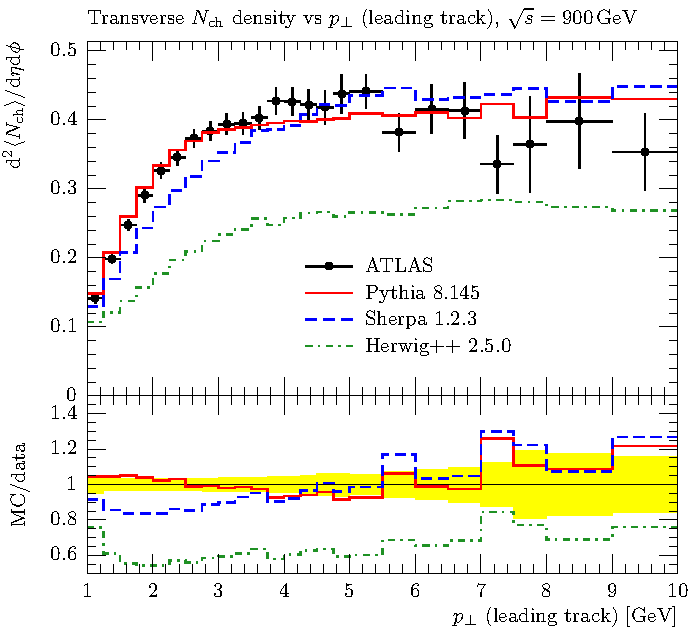
\includegraphics[scale=0.7]{mc-plots/ATLAS_2010_CONF_2010_081-cmp/ATLAS_2010_CONF_2010_081_d01-x02-y01}}
  \subfigure[Transverse $N_\text{ch}$ at 7~TeV]{\label{fig:cmp:mpi-ue-atlas7000-nch}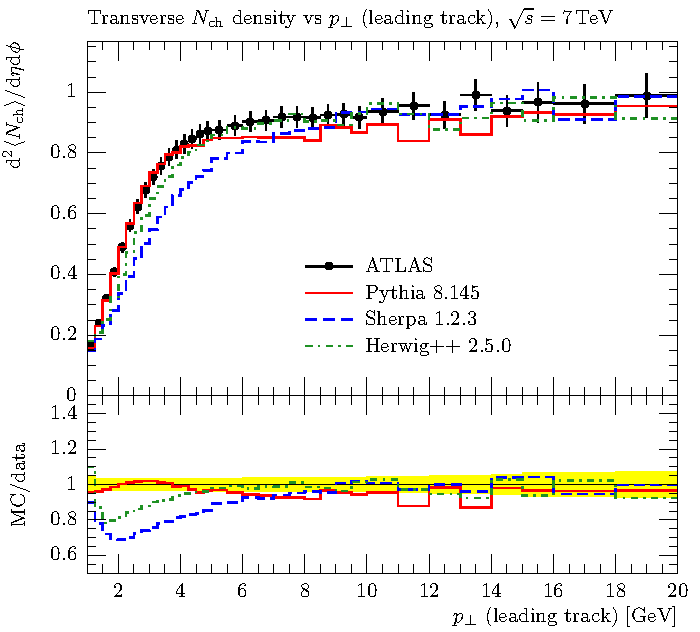
\includegraphics[scale=0.7]{mc-plots/ATLAS_2010_CONF_2010_081-cmp/ATLAS_2010_CONF_2010_081_d11-x02-y01}}
  \caption{ATLAS 900~GeV and 7~TeV underlying event observables, showing
    the dependence of MPI activity on the \pT of the leading charged
    particle in the event, with a charged particle \pT cut of
    $\pT > 500~\text{MeV}$, $|\eta| < 2.5$, $c\tau > 10\,\text{mm}$
    \cite{Aad:2010fh}. The MC description of
    these observables is dominated by the tuning of the MPI models, as
    described in \SecRef{sec:minim-bias-underly}. Up-to-date versions of
    these plots can be found at \url{http://mcplots.cern.ch/}.}
  \label{fig:cmp:mpi-ue-atlas-1}
\end{figure}

\begin{figure}[tp]
  \centering
  \subfigure[Transverse $\pT^\text{sum}$ at 900~GeV]{\label{fig:cmp:mpi-ue-atlas900-ptsum}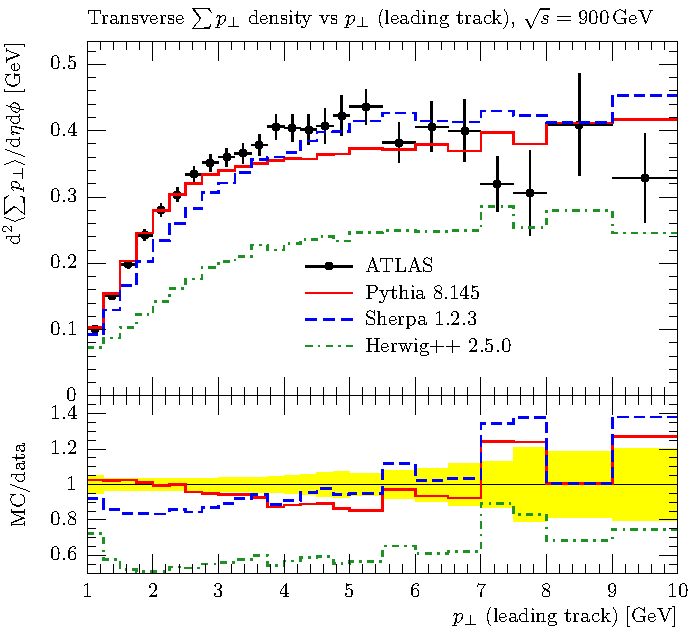
\includegraphics[scale=0.7]{mc-plots/ATLAS_2010_CONF_2010_081-cmp/ATLAS_2010_CONF_2010_081_d02-x02-y01}}
  \subfigure[Transverse $\pT^\text{sum}$ at 7~TeV]{\label{fig:cmp:mpi-ue-atlas7000-ptsum}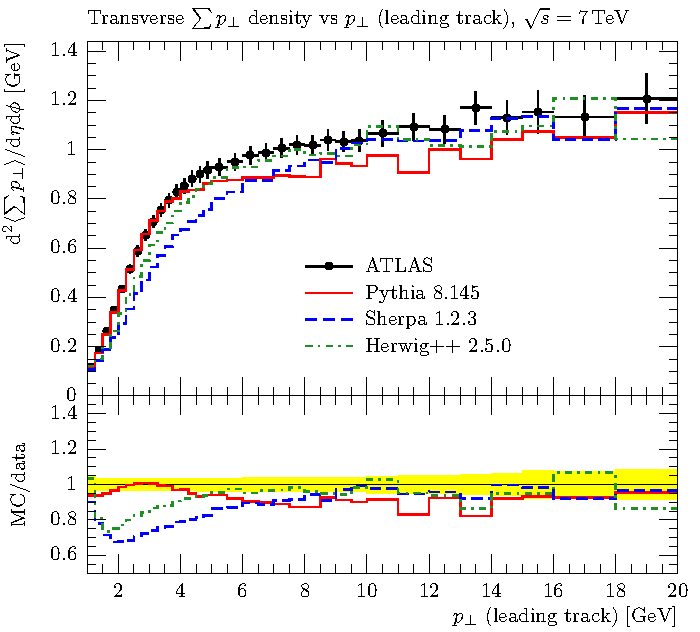
\includegraphics[scale=0.7]{mc-plots/ATLAS_2010_CONF_2010_081-cmp/ATLAS_2010_CONF_2010_081_d12-x02-y01}}
  \caption{ATLAS 900~GeV and 7~TeV underlying event observables, showing
    the dependence of MPI activity on the \pT of the leading charged
    particle in the event, with a charged particle \pT cut of
    $\pT > 500~\text{MeV}$, $|\eta| < 2.5$, $c\tau > 10\,\text{mm}$
    \cite{Aad:2010fh}. The MC description of
    these observables is dominated by the tuning of the MPI models, as
    described in \SecRef{sec:minim-bias-underly}. Up-to-date versions of
    these plots can be found at \url{http://mcplots.cern.ch/}.}
  \label{fig:cmp:mpi-ue-atlas-2}
\end{figure}

\begin{figure}[tp]
  \centering
  \subfigure[Transverse $\langle \pT \rangle$ vs. $N_\text{ch}$ at 900~GeV]{\label{fig:cmp:mpi-ue-atlas900-ptnch}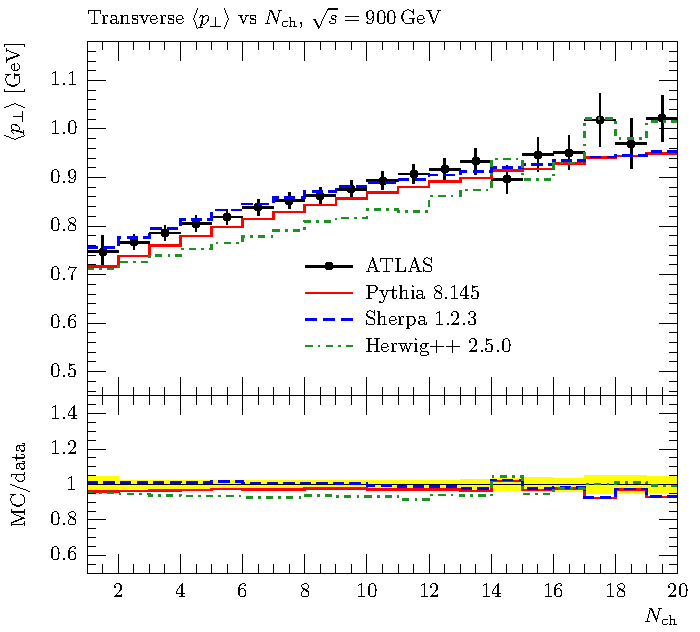
\includegraphics[scale=0.7]{mc-plots/ATLAS_2010_CONF_2010_081-cmp/ATLAS_2010_CONF_2010_081_d04-x02-y01}}
  \subfigure[Transverse $\langle \pT \rangle$ vs. $N_\text{ch}$ at 7~TeV]{\label{fig:cmp:mpi-ue-atlas7000-ptnch}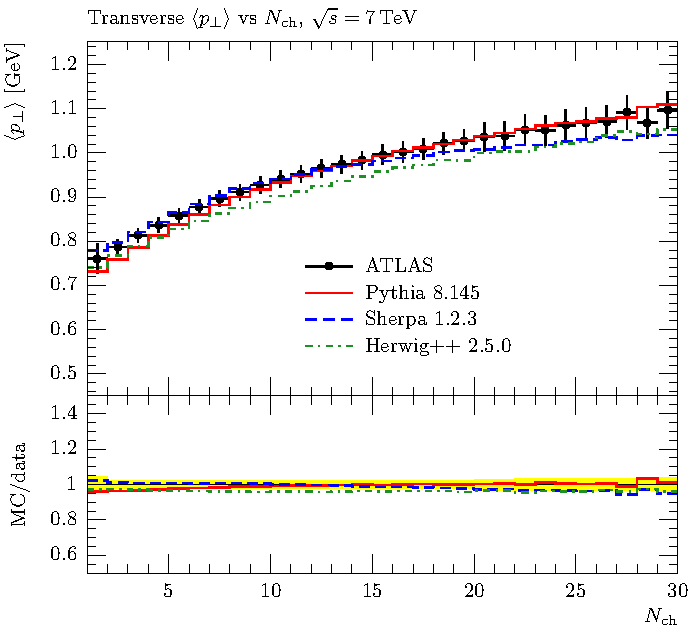
\includegraphics[scale=0.7]{mc-plots/ATLAS_2010_CONF_2010_081-cmp/ATLAS_2010_CONF_2010_081_d14-x02-y01}}
  \caption{ATLAS 900~GeV and 7~TeV underlying event $\langle \pT \rangle$
    vs. $N_\text{ch}$ correlation in the region transverse to the
    leading charged particle, with a charged particle \pT cut of
    $\pT > 500~\text{MeV}$, $|\eta| < 2.5$, $c\tau > 10\,\text{mm}$
    \cite{Aad:2010fh}. The MC description of
    these observables is dominated by the tuning of the MPI models, as
    described in \SecRef{sec:minim-bias-underly}. Up-to-date versions of
    these plots can be found at \url{http://mcplots.cern.ch/}.}
  \label{fig:cmp:mpi-ue-atlas-3}
\end{figure}

\begin{figure}[tp]
  \centering
  \subfigure[CDF~Run~2 transverse $\pT^\text{sum}$ in leading jet events at 1960~GeV]{\label{fig:cmp:mpi-ue-cdf2-ptsum}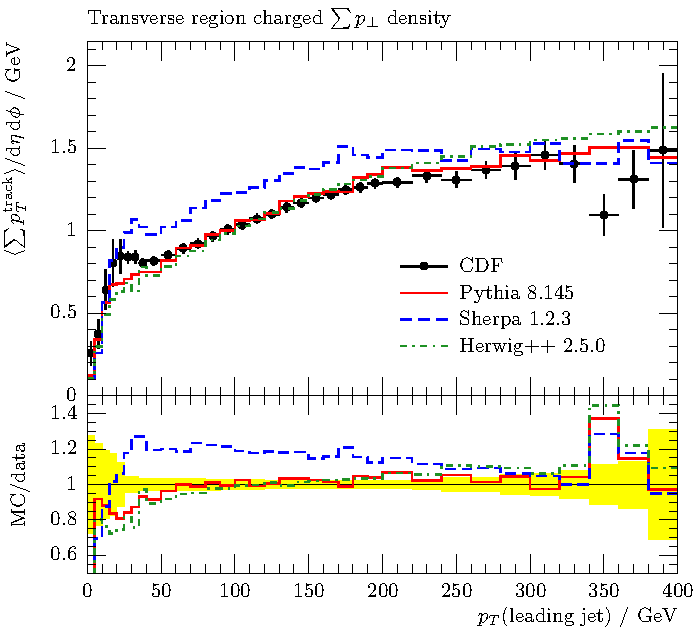
\includegraphics[scale=0.7]{mc-plots/CDF_2008_LEADINGJETS-cmp/CDF_2008_LEADINGJETS_d05-x01-y01}}
  \subfigure[CDF~Run~2 towards $\pT^\text{sum}$ in Drell-Yan events at 1960~GeV]{\label{fig:cmp:mpi-ue-cdf2-ptsum-drellyan}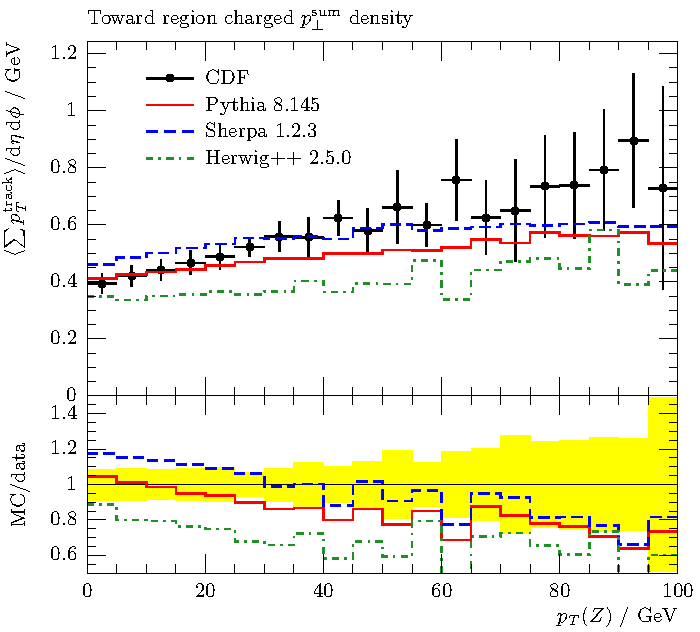
\includegraphics[scale=0.7]{mc-plots/CDF_2008_NOTE_9351-cmp/CDF_2008_NOTE_9351_d07-x01-y01}}
  \caption{CDF Run~2 underlying event profile observables: the $\pT^\text{sum}$
    is shown in the transverse region for leading jet events, and the towards
    region in Drell-Yan events \cite{Aaltonen:2010rm}. Up-to-date
    versions of these plots can be found at \url{http://mcplots.cern.ch/}.}
  \label{fig:cmp:mpi-ue-cdf}
\end{figure}

\begin{figure}[tp]
  \centering
  \subfigure[Summed out-of-event-plane $\pT$ \cite{Barate:1996fi}]{\label{fig:cmp:eeshapes-ptout}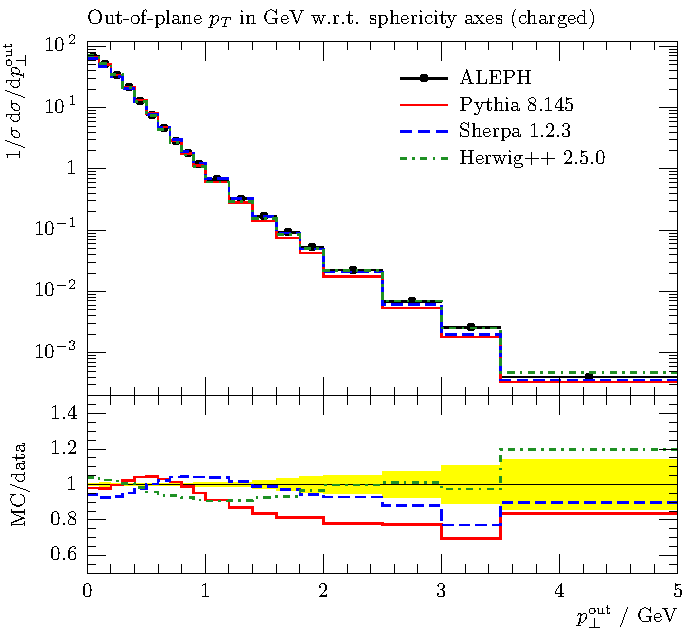
\includegraphics[scale=0.7]{mc-plots/ALEPH_1996_S3486095-cmp/ALEPH_1996_S3486095_d12-x01-y01}}
  \subfigure[$1-\text{Thrust}$ \cite{Heister:2003aj}]{\label{fig:cmp:eeshapes-thrust}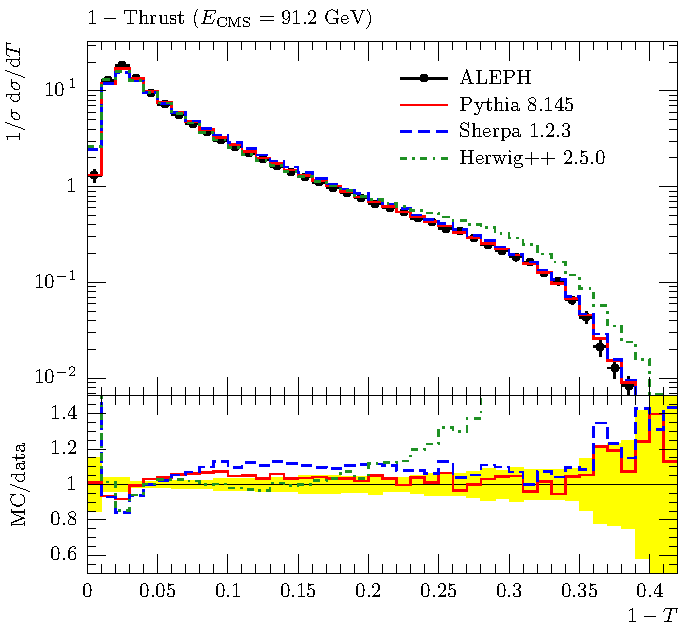
\includegraphics[scale=0.7]{mc-plots/ALEPH_2004_S5765862-cmp/ALEPH_2004_S5765862_d54-x01-y01}}\\
  \caption{\ee event shapes measured by ALEPH at 91\,GeV \cite{Barate:1996fi,Heister:2003aj}. Up-to-date versions of these plots can be found at \url{http://mcplots.cern.ch/}.}
  \label{fig:cmp:eeshapes}
\end{figure}

\begin{figure}[tp]
  \centering
  \subfigure[Differential 3-jet rate]{\label{fig:cmp:eeshapes-jety23}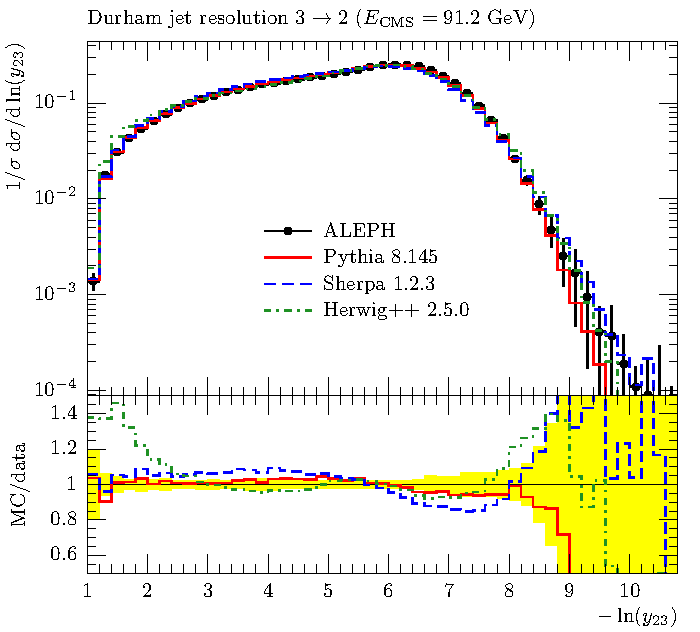
\includegraphics[scale=0.7]{mc-plots/ALEPH_2004_S5765862-cmp/ALEPH_2004_S5765862_d157-x01-y01}}
  \subfigure[Differential 5-jet rate]{\label{fig:cmp:eeshapes-jety56}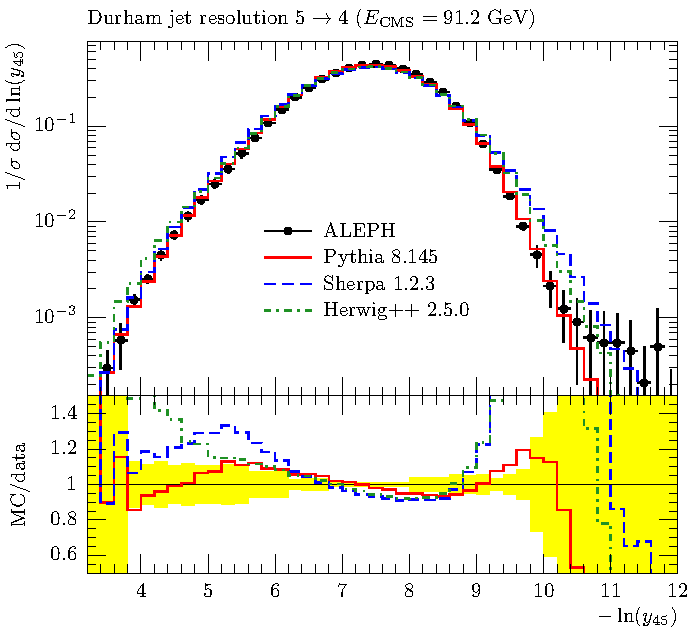
\includegraphics[scale=0.7]{mc-plots/ALEPH_2004_S5765862-cmp/ALEPH_2004_S5765862_d173-x01-y01}}
  \caption{\ee differential jet rates measured by ALEPH at 91\,GeV \cite{Heister:2003aj}.  The quantity $y_{n-1,n}$ is
    the value of the \kt-jet resolution at which $n$ jets are just
    resolved.  Up-to-date versions of these plots can be found at
  \url{http://mcplots.cern.ch/}.}
  \label{fig:cmp:eejetrates}
\end{figure}

\begin{figure}[tp]
  \centering
  \subfigure[D\O{} dijet azimuthal decorrelation \cite{Abazov:2004hm}]{\label{fig:cmp:dijet-azimdecorr}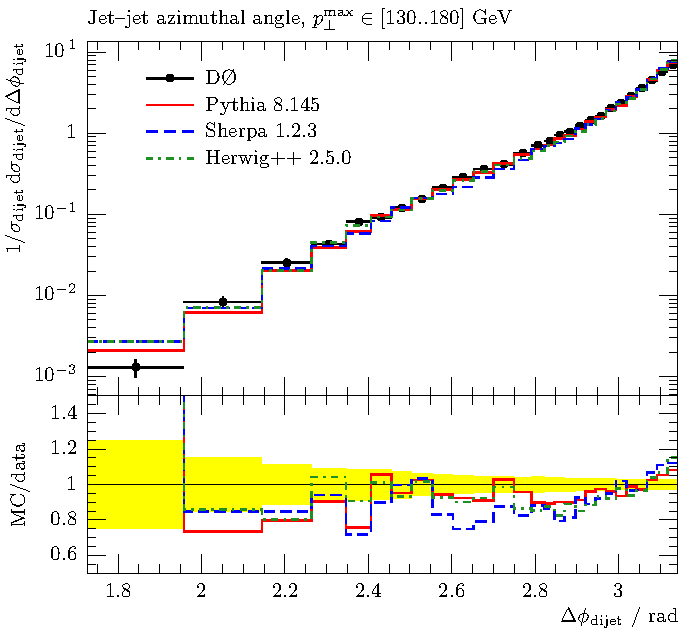
\includegraphics[scale=0.7]{mc-plots/D0_2004_S5992206-cmp/D0_2004_S5992206_d03-x02-y01}}
  \subfigure[Hadron collider jet shapes: CDF \cite{Acosta:2005ix}]{\label{fig:cmp:hadronic-jetshapes}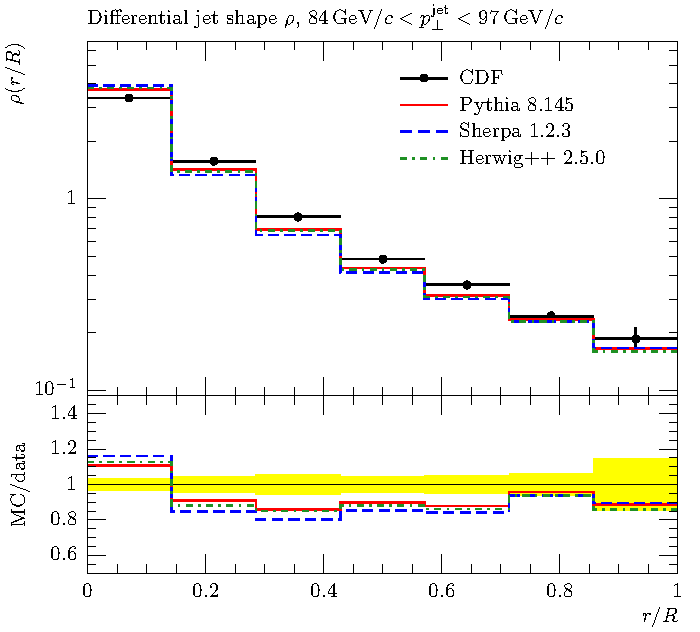
\includegraphics[scale=0.7]{mc-plots/CDF_2005_S6217184-cmp/CDF_2005_S6217184_d02-x01-y03}}
  \caption{Hadron collider shower-sensitive observables: dijet azimuthal
    decorrelation and jet shapes measured by D\O{} and CDF in Run~2 \cite{Abazov:2004hm,Acosta:2005ix}.
    The azimuthal decorrelation is a measure of
    the influence of three-jet configurations and shower emissions in disrupting
    a purely back-to-back two-parton configuration. Jet shapes measure the
    distribution of (transverse) momentum as a function of radius within jets.
    Up-to-date versions of these plots can be found at
    \url{http://mcplots.cern.ch/}.}
  \label{fig:cmp:ppshapes}
\end{figure}

\begin{figure}[tp]
  \centering
  \subfigure[LEP/SLD identified particle multiplicities \cite{Amsler:2008zzb}]{\label{fig:cmp:multis}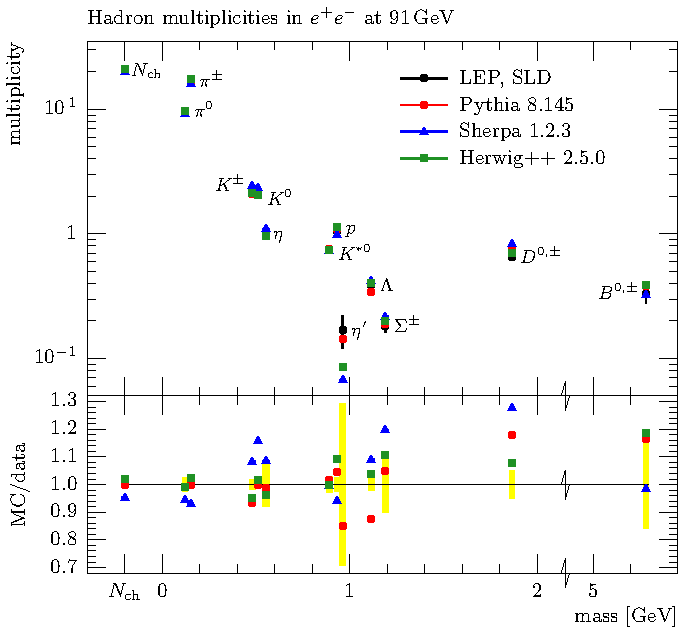
\includegraphics[scale=0.7]{mc-plots/PDG_HADRON_MULTIPLICITIES-cmp/PDG_HADRON_MULTIPLICITIES}}
  \subfigure[STAR identified particle mean $p_\perp$ \cite{Abelev:2006cs}]{\label{fig:cmp:particle-mean-pt}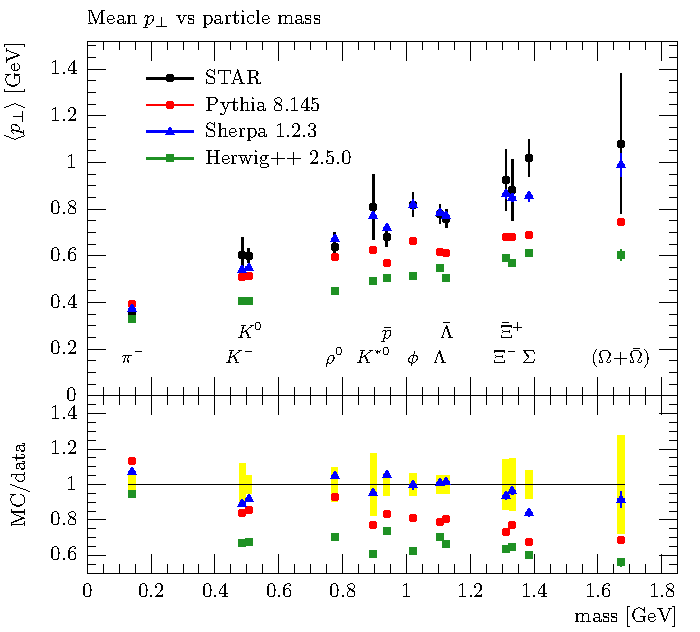
\includegraphics[scale=0.7]{mc-plots/STAR_2006_S6860818-cmp/STAR_2006_S6860818_d03-x01-y01}}
  \caption{Identified hadron multiplicities in $e^+e^-$ collisions at
    the $Z$ peak and $\langle \pt \rangle$ vs. particle mass in $pp$ collisions
    at 200\,GeV. These observables are determined primarily by the tuning
    of the hadronization models, both the flavour and kinematic aspects, but the
    overall multiplicities are also strongly dependent on the tuning of the
    parton showers (and MPI models, for the hadron collider observables).
    Up-to-date versions of these plots can be found at
    \url{http://mcplots.cern.ch/}.}
  \label{fig:cmp:idparticle-rates}
\end{figure}

\begin{figure}[tp]
  \centering
  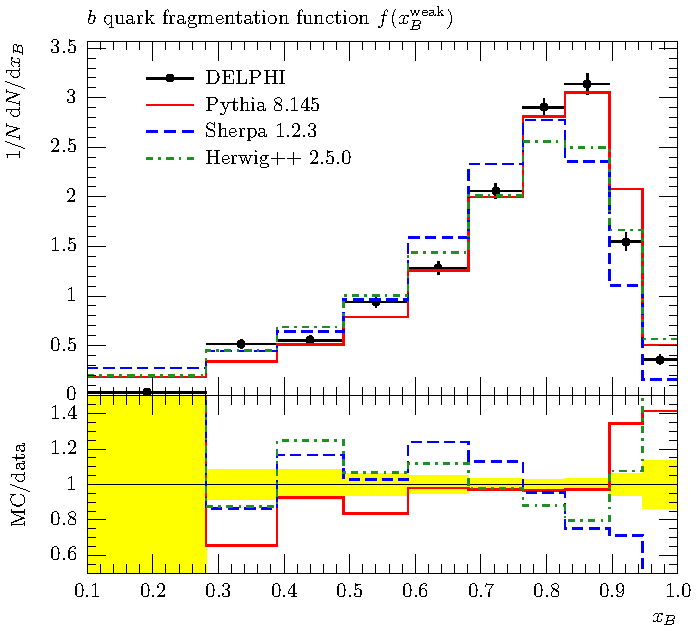
\includegraphics[scale=0.7]{mc-plots/DELPHI_2002_069_CONF_603-cmp/DELPHI_2002_069_CONF_603_d02-x01-y01}
  \caption{DELPHI $B$ fragmentation function $x_B = 2 E_B / \sqrt{s}$
    for weakly decaying $b$ hadrons \cite{Barker:2002}. Most Monte Carlo
    models apply a special fragmentation function treatment to heavy
    quarks, but this observable is not entirely decoupled from light
    quark fragmentation parameters. An up-to-date version of this plot
    can be found at \url{http://mcplots.cern.ch/}.}
  \label{fig:cmp:bfragfunction}
\end{figure}

\begin{figure}[tp]
  \centering
  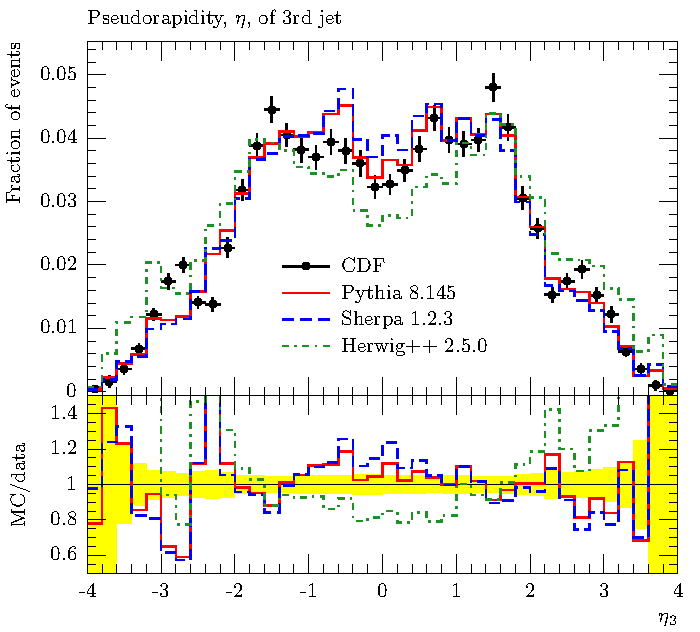
\includegraphics[scale=0.7]{mc-plots/CDF_1994_S2952106-cmp/CDF_1994_S2952106_d03-x01-y01}
  \caption{CDF's evidence for colour coherence in $p\bar{p}$ collisions at
    $\sqrt{s} = 1.8$~TeV \cite{Abe:1994nj}. The pseudorapidity of the
    third jet is plotted, uncorrected for detector effects, with the
    \herwigpp, \pythiaeight and \sherpa Monte Carlo generators. All
    these generators include colour coherence effects via either angular-ordered
    parton showers (\herwigpp) or transverse-momentum-ordered dipole showers
    (\pythiaeight, \sherpa),  and hence correctly exhibit a dip at central
    rapidity. The correlated fluctuations between MC samples are due to
    statistical errors on the detector-smearing correction factors taken
    from the CDF paper. An up-to-date version of this plot can be found
    at \url{http://mcplots.cern.ch/}.}
  \label{fig:cmp:cdf-colour-coherence}
\end{figure}


% Local Variables:
% mode: LaTeX
% TeX-master: "../mcreview"
% End:
